\section{Hintergrund und Kontext}
Durch die zunehmende Globalisierung und Digitalisierung wird die Gesellschaft der Gegenwart und Zukunft geprägt. Der Ausbau von Hochgeschwindigkeitsnetze und die globale Corona-Pandemie haben diese Entwicklung noch einmal beschleunigt. Immer mehr Unternehmen erkennen die Potenziale der Digitalisierung und stellen ihre Geschäftsprozesse um. Ganze Wertschöpfungsketten werden auf cloudbasierte Umgebungen umgestellt. Angefangen bei der Kommunikation, über Beschaffung und Produktion bis zum Verkauf der Waren und Dienstleistungen, vergleiche mit \parencite[Seite 21 ff.]{banholzer-2020} und \cite{oswald-2022}. In allen Stufen der Prozesse kommen webbasierte Anwendungen zum Einsatz, um die Kommunikation der Anwender mit den Systemen zu ermöglichen oder Schnittstellen für die Datenübertragung zwischen den verschiedenen Systemen zu gewährleisten. Durch wachsende Anzahl von Web-Anwendungen wächst auch der Druck für die Entwicklungsfirmen, ihre Anwendungen den schnell und oft wechselnden Kundenanforderungen anzupassen.\vspace{0.2cm}

Durch diesen Prozess getrieben, müssen Entwicklungsfirmen in immer kürzeren Release-Zyklen Softwarekomponenten hinzufügen und vorhandene erweitern. Gleichzeitig wachsen aber auch die Anforderungen an Stabilität und Sicherheit der cloudbasierten Anwendungen, sowie der Bedarf an kostengünstigeren IT-Abläufen (Beweis fehlt). Ein weiteres Problem ist der wachsende Fachkräftemangel in der Wirtschaft und die damit verbundenen steigenden Gehälter der Entwickler (Beweis fehlt).\vspace{0.2cm}

Die Verwendung künstlicher Intelligenz bei der Programmierung gewinnt immer mehr an Bedeutung. Eine Technologie die im besonderen Maße an dieser Entwicklung beteiligt ist, sind die Large Language Models. Insbesondere mit der Veröffentlichung vom ChatGPT wurde hier ein regelrechter Hype um die \acrshort{LLM}s ausgelöst. Diese Modelle erlauben eine Softwareentwicklung mit natürlicher Sprache. Tiefe Kenntnisse der verwendeten Programmiersprache sind nicht mehr in dem Maße erforderlich, wie ohne LLMs.\vspace{0.2cm}


\section{Problemstellung}
So groß der Hype um Künstliche Intelligenz auch sein mag, zurzeit kann KI nicht alle Anforderungen selbstständig lösen. Dies sollte auch bei der Verwendung von KI generierten Inhalten und Programmcodes beachtet werden.

\epigraph[
	source={Vattenfall Online},
	etc={ KI für Unternehmen – die Grenzen der KI},
	author and source indent=0.5cm,
	dash=,
	after skip=0.5cm
]{KI denkt nicht, KI trifft keine Entscheidungen. Eine KI antwortet auf eine Eingabe nicht mit der besten Antwort, sondern mit der Wahrscheinlichsten.}

Der Mensch muss die generierten Ergebnisse überprüfen, ehe erstellte Programmcodestücke in vorhandene Programme eingefügt und in Produktionsumgebungen implementiert werden.\vspace{0.3cm}

Viele Entwickler setzen auf Chatbots, wie ChatGPT oder Gemini zur Generierung von Code, wie eine Umfrage von \textit{stackoverflow} vom Mai 2024 zeigt \cite{noauthor_developers_2024}. Gleichzeitig wachsen auch die technischen Schulden bei Softwareprojekten, da diese Modelle nicht für die Entwicklung von Software optimiert sind (Beweis fehlt).\vspace{0.2cm}

%\subsection{Herausforderungen bei der Entwicklung von Webanwendungen}

%\subsection{Potenzial von LLMs in der Webentwicklung}


\section{Stand der Forschung}
In \cite{jiang-2024} wird eine bis dato fehlende Literaturrecherche zum Thema Codegenerierung durch große Sprachmodelle bemängelt, was in dieser Arbeit nachgeholt wird und haben im Juni 2024 Literatur zusammengetragen, welche sich mit Codegenerierung befasst.\vspace{0.2cm}

Um die Prompts im Ingenieurswesen zu optimieren, wird in \cite{velasquez-henao-2023} die GPEI Methodik vorgeschlagen, welche aus vier Schritten besteht. Zuerst wird das Ziel definiert, dann ein Entwurf der Anforderung, im Anschluss die Bewertung gefolgt von Iterationen.\vspace{0.2cm}

Es gibt Bestrebungen kleinere Modelle die auf Codegenerierung spezialisiert sind, mit den großen Sprachmodellen zu testen, so auch in \cite{mishra-2024}. Hier werden die Modelle als \glqq Granite Code Models\grqq -Familie zusammengefasst. Eine weitere Arbeit die sich mit kleinen Modellen, die besonders für das Generieren von Code trainiert wurden, befasst sich die Arbeit \cite{lozhkov-2024} mit StarCoder 2 betrachtet.\vspace{0.2cm}

Der wissenschaftlicher Artikel \cite{nataraj-2024} befasst die sich ebenfalls mit der Web-Entwicklung mittel GPT-3. Hierbei wird die Verwendung von Generativ Adversarial Networks (GANs) vorgeschlagen, ein neuer Ansatz, mit der die Nachbearbeitung minimiert und die Codequalität optimiert wird.

\section{Zielsetzung und Forschungsfragen}
Das Ziel in der Softwareentwicklung war und ist die Optimierung des Entwicklungsprozesses, um Ressourcen und Kosten einzusparen und dadurch einen Wettbewerbsvorteil zu erlangen. Die steigende Nachfrage von Cloud-Anwendungen steigt auch der Optimierungsdruck in diesem Bereich besonders stark.\vspace{0.2cm}

Vor diesem Hintergrund lässt sich die Zielsetzung bereits aus dem Titel \glqq \textit{Evaluierung und Optimierung von Large Language Models für die Entwicklung von Webanwendungen}\grqq \ dieser Arbeit herleiten. Sie untersucht die Möglichkeiten mit natürlicher Sprache Code zu generieren. In dieser Arbeit wird, wie auch in \cite[vgl. Seite 2]{jiang-2024} Language-to-Code, kurz NL2Code verwendet. Diese Arbeit soll eine Auswahl von Modellen evaluieren und dessen Brauchbarkeit für die Softwareentwicklung aufzeigen. Um die Antworten der Modelle zu optimieren, soll eine Evaluation von Methodiken erfolgen, bei der deren Anwendung auf die Modelle eine Verbesserung der Antworten ersichtlich ist. Des Weiteren soll gezeigt werden, ob und wie weit sich der Prozess der Codegenerierung automatisieren lässt und ob einige Programmiersprachen, die in der Webentwicklung Verwendung finden, besser unterstützt und geeignet sind als andere und somit zu bevorzugen sind.\vspace{0.2cm}

Die vier Ziele dieser Arbeit lassen sich in den folgenden kurz formulierten Sätzen zusammenfassen,

\begin{itemize}
	\item[Z1] Welche Modelle eigenen sich für die Softwareentwicklung.
	\item[Z2] Welche Methodiken helfen die Qualität der Antworten von Modellen zu verbessern.
	\item[Z3] Wie weit lässt sich die Verwendung von großen Sprachmodellen, für die Erstellung von Webanwendungen automatisieren.
	\item[Z4] Sind einige Programmiersprachen für die Codegenerierung besser geeignet als andere.
\end{itemize}

%-------------------------------------------------------------------------------------------------


\subsection{Auswahl der LLMs}
Die folgenden Modelle werden getestet und die Ergebnisse anschließend evaluiert.
\begin{table}
	\begin{tabular}{|l|c|c|c|c|l|}
		\hline
		\textbf{Modell} & \textbf{Parameter} & \textbf{Größe} & \textbf{offen} & \textbf{Ausführung}  & \textbf{Benchmark} \\
		\hline
		Qwen2.5-coder     & 32b &  19 GB & X & lokal  & HumenEval-XL \\
%		CodeGeeX          &  9B & & & lokal & HumenEval-XL \\
		Deepseek-coder-V2 & 16B & 8,9 GB & X & lokal  & HumenEval-XL \\
		Llama3.1-Claude   &  8b & 4,7 GB & X & lokal  & HumenEval-XL \\
		Llama3.2          &  3b & 2,0 GB & X & lokal  & HumenEval-XL \\
		Codellama         & 13b & 7,4 GB & X & lokal  & HumanEval-XL \\
%		ChatGPT3.5        & & & & online & HumenEval-XL \\
		Gemini Flash 1.5  & k.A.& k.A.   & - & online & HumenEval-XL \\
%		Opus              & & & & online & HumenEval-XL \\
%		Claude 3          & & & & online & HumenEval-XL \\
		\hline
		\multicolumn{6}{|l|}{In Planung, wenn ich es schaffe} \\
		\hline
		Llama3.3          & 70b &  43 GB & X & lokal  & HumanEval-XL \\
		\hline
	\end{tabular}
\end{table}

%\begin{tcolorbox}[
%	enhanced,
%	colback=yellow!5!white,
%	colframe=yellow!75!black!50,
%	title= Wird noch im Verlauf der Arbeit geändert
%	]
%	Als Referenzen kommen ChatGPT3.5 und das aktuelle Google Sprachmodell der Gemini-Familie zum Einsatz.\vspace{0.2cm}

%	Als lokale Modelle werden zurzeit deepseek-coder-v2, llama3.1-claude und llama3.2 verwendet. Diese Modelle kommen auch zum Einsatz, für die Orchestrierung und die Multi-Agenten-Systeme.\vspace{0.2cm}
	
%	Das neue Model Mistral Lage 2 (Links: \href{https://mistral.ai/news/mistral-large-2407/}{Mistral Large 2 | Mistral AI} und \href{https://the-decoder.de/mistral-large-2-soll-meta-llama-3-in-sachen-effizienz-schlagen-und-der-llm-ozean-wird-roter/}{Mistral Large 2 | the-decoder.de} [gelsen am: 03.11.2024]) soll in Sachen Coding mit Modellen wie GPT-4o, Claude 3 Opus und Llama 3 mithalten können. (Gibt es auch von \href{https://ollama.com/library/mistral-large}{mistral-lage | ollama Models})\vspace{0.2cm}
	
%	Evtl. werden die Granite Code Models aus \cite{mishra-2024} auch getestet.
%\end{tcolorbox}

%-------------------------------------------------------------------------------------------------


\subsection{Prompt-Engineering}
% https://dev.to/pavanbelagatti/prompt-engineering-for-developers-a-complete-guide-1kca
\begin{tcolorbox}[
	enhanced,
	colback=yellow!5!white,
	colframe=yellow!75!black!50,
	title= Wird noch im Verlauf der Arbeit geändert
	]
	Ob alle in Kap. \ref{subsec:prompt_technics} vorgestellten Prompt-Techniken Verwendung finden, steht zurzeit noch nicht fest. Evtl. kommen andere hinzu.
\end{tcolorbox}

\textbf{Evaluierung der Ergebnisse}\vspace{0.2cm}

Bei der Evaluierung großer Sprachmodell hinsichtlich des generierten Codes, gibt es einige Herausforderungen. Herkömmliche Methoden, wie BLUE-Score misst die Textähnlichkeiten nicht aber die funktionale Korrektheit des Codes und vernachlässigt auch den Kontext, in dem der Code erstellt wurde. Ein generierter Code kann in seiner Lösung stark von einer vorgegebenen Beispiellösung abweichen, trotzdem aber seine Funktionalität erfüllen. Menschliche Programmierer würden das mit verschiedenen Unit-Tests überprüfen, aus diesem Grund sollte der Code mit einer weiteren Methode geprüft werden.\vspace{0.2cm}

HumanEval-Benchmark and pass@k-Metrik

\href{https://deepgram.com/learn/humaneval-llm-benchmark}{Einstieg}

\href{https://paperswithcode.com/sota/code-generation-on-humaneval}{Modell}

\href{https://huggingface.co/datasets/openai/openai_humaneval}{Huggenface}

\href{https://github.com/openai/human-eval/tree/master}{Github}

\href{https://arxiv.org/abs/2107.03374}{Einführendes Paper}

%-------------------------------------------------------------------------------------------------


\subsection{Benchmark für LLM}
Als Benchmark für die Bewertung der großen Sprachmodelle wird der HumanEval-XL verwendet, welche unter \href{https://github.com/FloatAI/humaneval-xl/tree/main}{https://github.com/FloatAI/humaneval-xl/tree/main} heruntergeladen werden können. Der Benchmark besteht aus Prompt, die wie folgt aufgebaut sind,

\begin{itemize}
	\item \textbf{task\_id}: Kennung der Datenprobe
	\item \textbf{prompt}: Anfrage für das Modell, Funktionsheader und Docstring
	\item \textbf{entry\_point}: Einstiegspunkt für den Test
	\item \textbf{description}: Beschreibung der Aufgabe
	\item \textbf{language}: Kennung der Programmiersprache
	\item \textbf{canonical\_solution}: Lösung für das Problem
	\item \textbf{natural\_language}: Ländersprache in der Datei
\end{itemize}

Durch diesen Aufbau werden neben dem eigentlichen Prompt ein Test, eine vorgeschlagene Lösung mitgeliefert, sowie weitere Metadaten mit geliefert. Die Abbildung \ref{img:code_generation_humaneval} zeigt den Aufbau und damit alle wichtigen Bereiche des Benchmark-Tests.

\begin{figure}[!ht]
	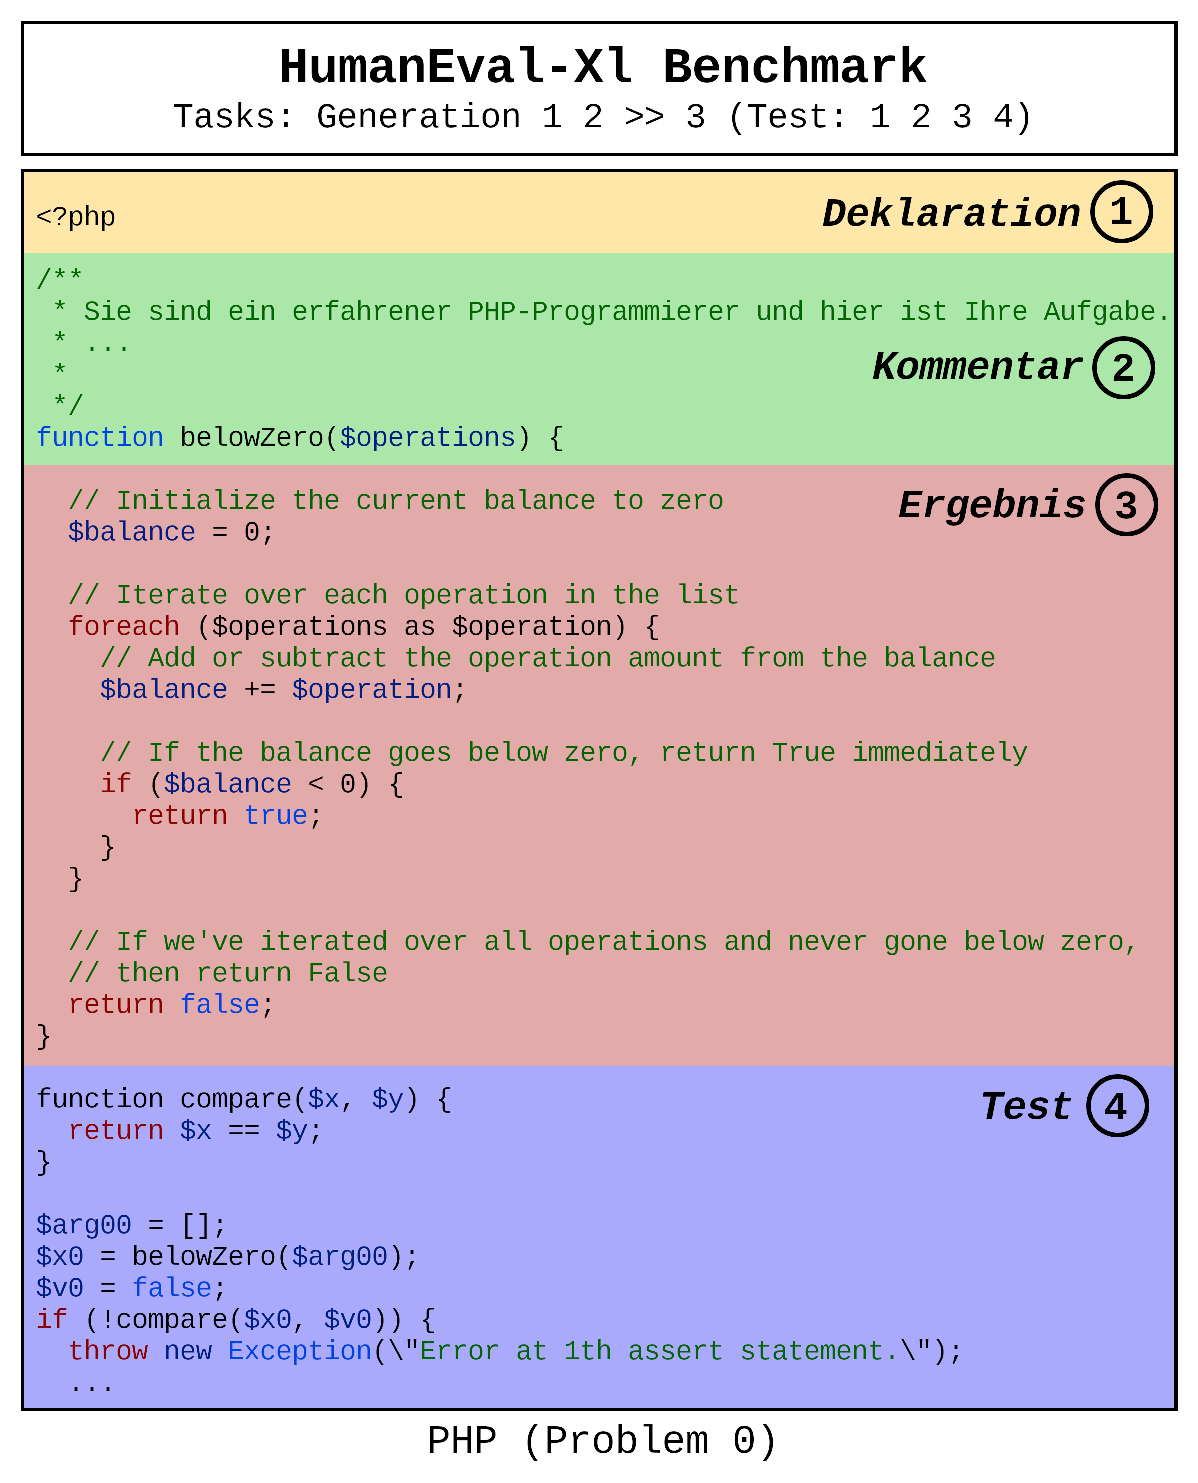
\includegraphics[width=0.8\textwidth]{content/chapter_intruduction/images/code_generation_humaneval_x.eps}
	\centering
	\caption{Codegeneration}
	\label{img:code_generation_humaneval}
\end{figure}
%-------------------------------------------------------------------------------------------------


\section{Aufbau der Arbeit}
Ein paar Worte zum Aufbau dieser Arbeit. Um ein grundlegendes Verständnis für diese Arbeit zubekommen, werden im Kapitel \ref{chap:basics} die Grundlagen besprochen.\vspace{0.2cm}

Im Kapitel \ref{chap:state_of_research} wird der aktuelle Stand der Forschung vorgestellt und Erkenntnisse anderer Arbeiten diskutiert. Die Implementierung der Test LLMs wird in Kapitel \ref{chap:implementation} besprochen und in Kapitel \ref{chap:evaluation} die Ergebnisse evaluiert.\vspace{0.2cm}

Die negativen und positiven Erfahrungen und Herausforderungen werden in Kapitel \ref{chap:lessons_learned} aufgegriffen und Lösungsansätze vorgeschlagen, die in den nachfolgenden Kapiteln vorgestellt werden.\vspace{0.2cm}

Bevor in Kapitel \ref{chap:conclusion} auf mögliche Folgearbeiten eingegangen wird, gibt es in Kapitel \ref{chap:application_scenarios} Anwendungsszenarien, die auf den zuvor gewonnen Ergebnissen aufbauen und vorgestellt werden.


\section{Abgrenzung}
In dieser Arbeit fokussiert sich die Betrachtung auf den Bereich der Webanwendungsentwicklung und deren verwendete Programmiersprachen. Parallelen zu anderen Anwendungsbereichen, wie beispielsweise Desktop-Anwendungsentwicklung werden hier nicht expliziert betrachtet können aber durchaus vorkommen.\vspace{0.2cm}

Auch wenn rechtliche und ethische Überlegungen einen wichtigen Aspekt in Umgang mit Künstlicher Intelligenz darstellt, wird dies in dieser Arbeit nicht betrachtet. Es gibt hinreichend Literatur zu diesen Themen, die in dieser Arbeit Beachtung finden, es wird aber nicht explizit darauf eingegangen.\vspace{0.2cm}

\begin{tcolorbox}[
	enhanced,
	breakable,
	colback=red!5!white,
	colframe=red!75!black!50,
	title= Mein roter Faden: noch was zum Testen
	]
	Ein Tool zur Orchestrierung von Multi-Agenten-Systemen \href{https://community.openai.com/t/introducing-swarm-js-node-js-implementation-of-openai-swarm/977510}{OpenAI Swarm}, gefunden auf \href{https://karrierewelt.golem.de/blogs/karriere-ratgeber/bot-belegschaft-mit-entlastungspotenzial-ki-agenten-fur-den-arbeitsalltag-in-der-testphase-1}{Golem | Karrierrewelt}.
\end{tcolorbox}
